\section {Implementation}

We implemented two commenting systems as classical client/server web-applications. The first commenting system is MindMargin with anchored comments on a horizontal infinite scroll next to the reference medium. The second commenting system is a traditional vertical interface. Users interact with the clients as a front-end system using a web browser. The clients communicate with the server back-end using AJAX to a) request existing data or b) persist new data. The server reads and stores data in a relational database.

\subsection{Front-end}
The client interfaces consist of clean user interfaces to avoid design clutter and distraction. Figure \ref{fig:frontend} shows the MindMargin system in action. The application is split into two sides: The reference media on the left and and an adjacent commenting system on the right. The commenting system displays comments in a horizontal infinite scroll. Thus, an unrestricted amount of comments can be linked to the reference media. Navigation within the infinite scroll component can be performed via mousewheel interaction (either left/right or top/down scrolling with the same effect) or by adjustment of a slider on the bottom of the right split screen. Comments are anchored to the horizontal reference point of the media by thin dotted lines. If a comment has replies, a dropdown button appears on the comment's footer. Lighter in color, replies to comments appear vertically under their comment when the button is clicked. This arrangement optimizes horizontal real estate by reserving horizontal space for parent comments. Finally, while navigating through the infinite scroll, the reference medium remains fixed on the left for quick reference against referential comments and replies.

\begin{figure}
\centering
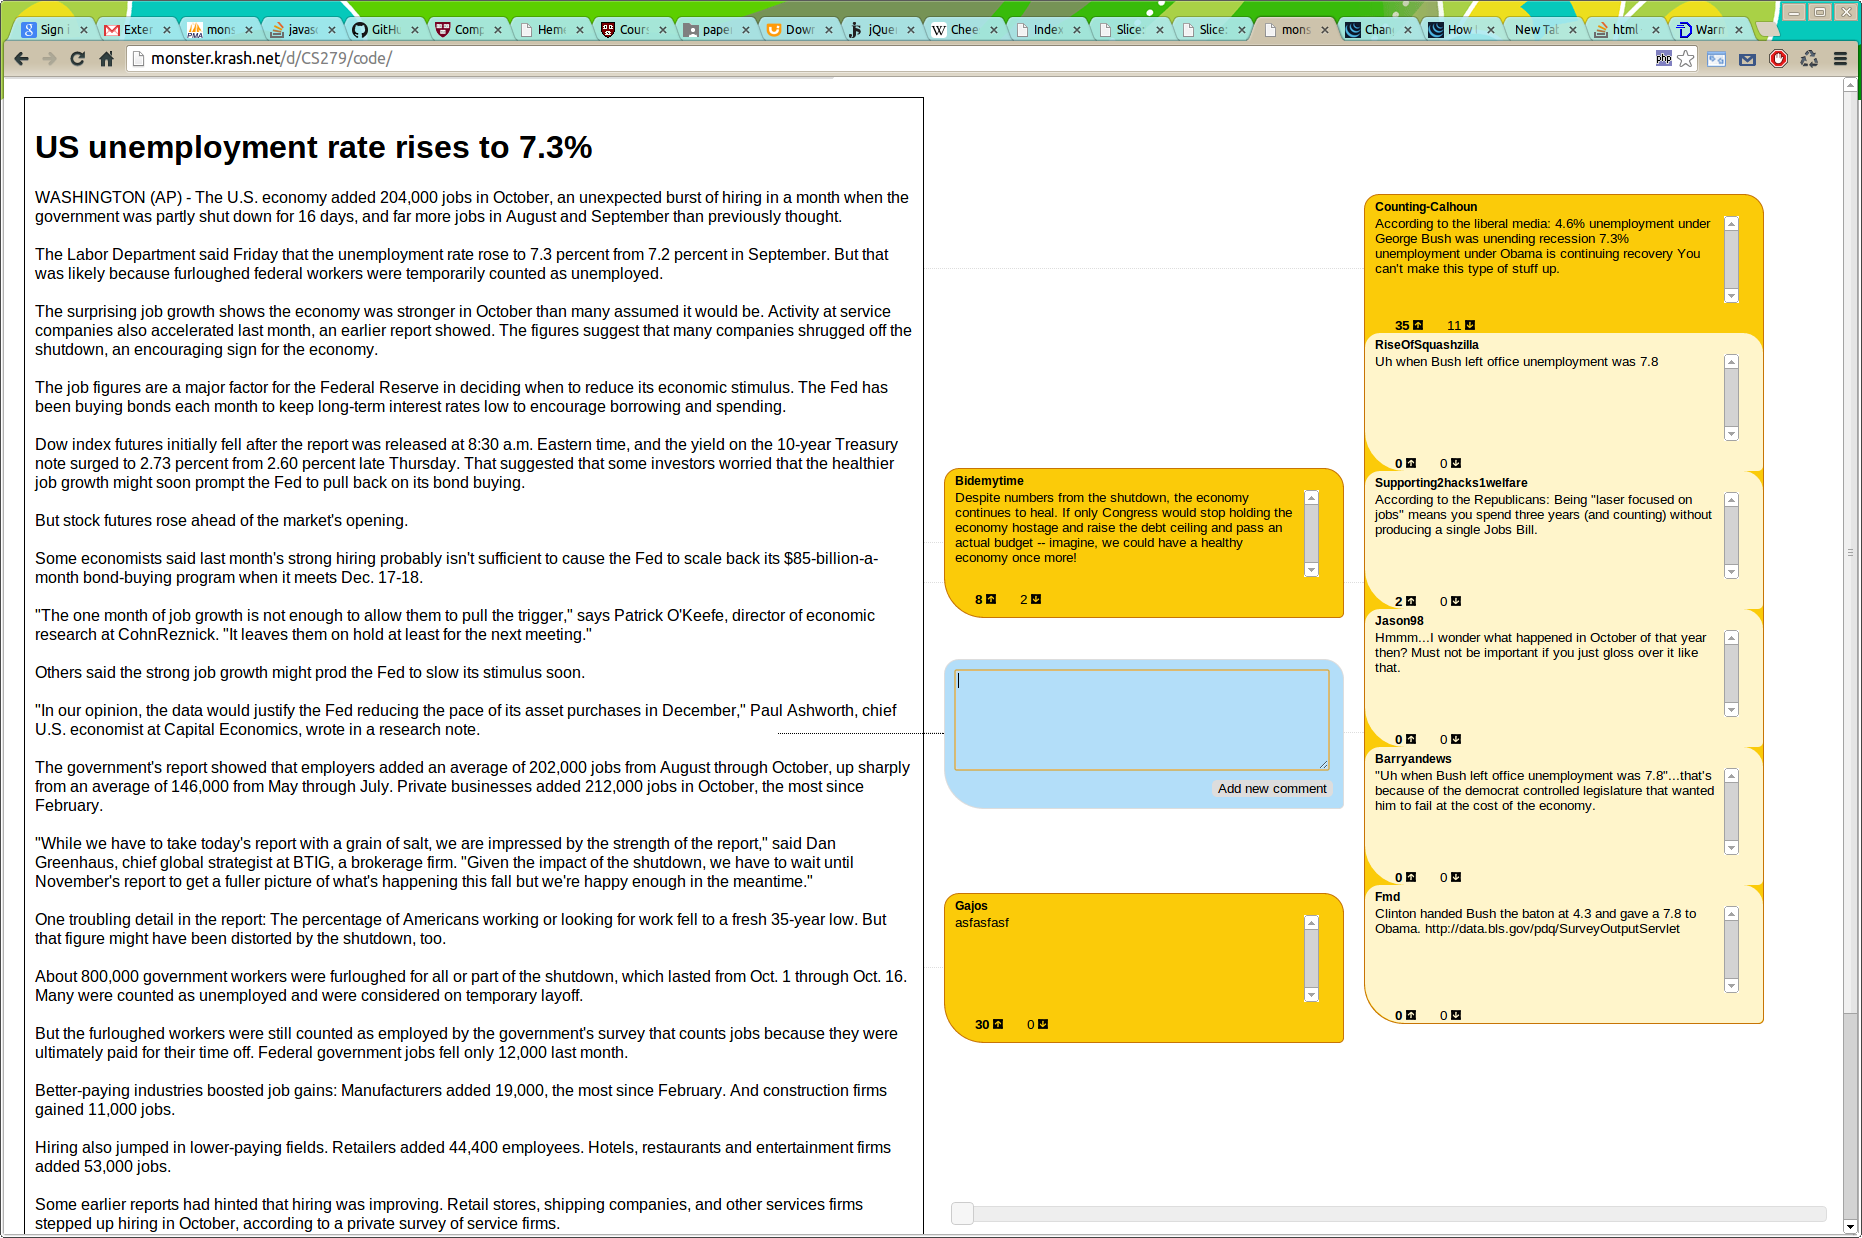
\includegraphics[scale=0.3]{mindmargin.png} 
\caption{The MindMargin system consists of a web client (shown here) and a server side back-end.}
\label{fig:frontend}
\end{figure}

Figure \ref{fig:traditional} shows the traditional vertical commenting system. The reference media appears first and on top of the commenting system that follows below. Navigation within the article as well as within the comments can be performed via top/down scrolling. The organization of replies and up- and down-voting is similar to the MindMargin prototype.

\begin{figure}
\centering
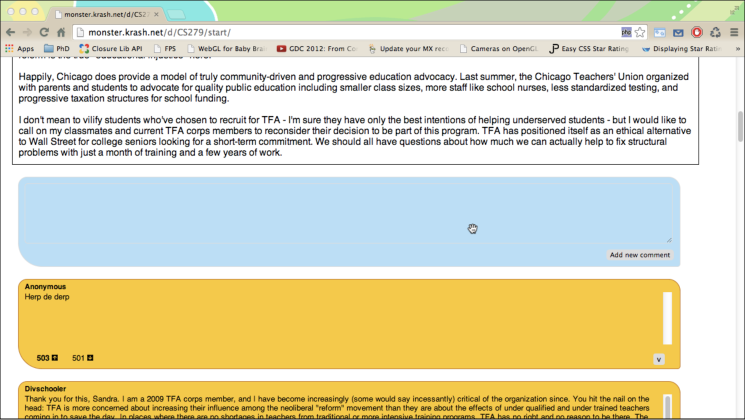
\includegraphics[scale=0.3]{traditional.png} 
\caption{The traditional comment system with a vertically ordered design.}
\label{fig:traditional}
\end{figure}

The front-ends were written in JavaScript using the popular jQuery and jQuery UI libraries. A model-view-controller pattern was chosen to structure the application code base. The user interface itself were created to adjust responsively to any window size.

\subsection{Back-end}
The server component of MindMargin and the traditonal system was written in PHP and communicates with the front-end and a relational database. Communication with the front-end is ensured by providing a REST-API which can be called via AJAX. The entity model of the client is replicated on the server. Data is read and stored using a custom and fully generalized object-relational-mapper. We chose MySQL for our database with a table each for users and comments.

Throughout the implementation, we followed an iterative approach to programming our software. The developer team was small. All developed code is released under the BSD open source license on github.